\section{Results}
The finished system implementation can be found at Github under \emph{https://github.com/Modular-Design}.
To support the multifunctional design process, the proposed solution has been focusing on two main capabilities,
which are separately tested and demonstrated below.
\subsection{Solving Complex Dependencies}
The first capability of the introduced system is 
to solve complex interactions and iterations loops that are characterized by a certain degree of non-linearity.
Therefor a material hoists is chosen, due to the fact that the motor weight adds 
to the overall weight of the lift (Fig. \ref{pic:lift_model}), 
hence causing a dependency loop.
With current methods, eigenweight problems in the part design are often simplified 
by overestimating the total load on the motor.
This results in a higher safety tolerance, but also increases the overall weight.
In cases where mass reduction is crucial like in aircraft and space applications, this is often not an option.
\begin{figure}[h]
    \centering
    \begin{subfigure}[b]{0.55\textwidth}
        \centering
        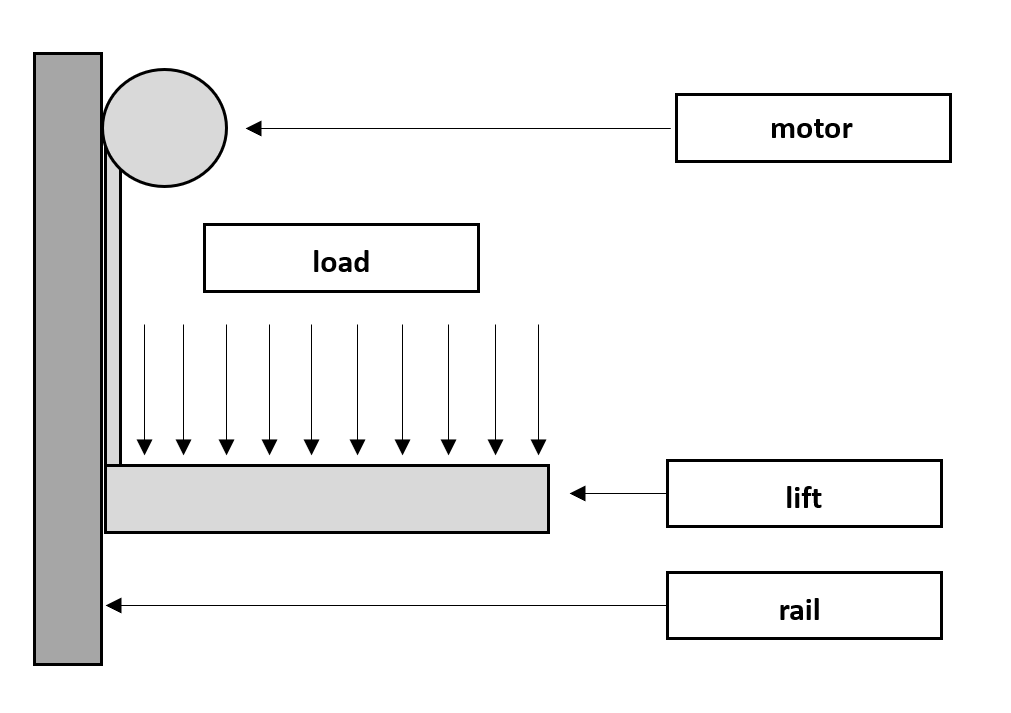
\includegraphics[width=\textwidth]{pics/500Z_model.png}
        \caption{\label{pic:lift_model} Model of a material lift.}
    \end{subfigure}
    \hfill
    \begin{subfigure}[b]{0.95\textwidth}
        \centering
        \includegraphics[width=\textwidth]{pics/_lift.pdf}
        \caption{\label{pic:lift_solu} Implementation of the design process.}
    \end{subfigure}
    \caption{\label{pic:lift} Designing of a material lift with the introduced framework.}
\end{figure}\\
Modelling the complex interaction of the hoist parts with the developed software allows to automatically update, change and test the current configuration.
Following the guidelines for light weight design process, the simplified model is broken down into several process, each describing the individual parts and 
their influence on different parameters of the hoist (Fig. \ref{pic:lift_solu}).\\
The motor process in Figure \ref{pic:lift} represents the selection process of a new motor, 
based on the minimum torque, RPM, power or maximum mass.
Realistically, determining the motor properties would be conducted by searching in a database, 
but open motor databases have many restrictions.
To keep the system simple and intuitive 
it was decided to determine the new motor based on a simple motor model.\\
Besides the motor, the designing of the baseplate is crucial to the overall structural integrity.
During the design process this is taken into account, by using two systems to represent separate aspects of the baseplate:\\
The CAD-Base is used to digital model the plate and change certain dimensions (Fig. \ref{pic:lift}).
This results in a CAD file being generated, which is then transferred to the simulation process.
There the inserted loads are applied to the model and the relevant stresses are computed.\\
The three main modules are distributed over the system and been accessed via a network communication.
To help modeling the complex functional dependencies additional math modules are used.
Due to lower hardware requirements, math modules are often provided locally.\\
Additionally to the high number of interactions, the safety margin was reduced to a value of 1.2 to 
artificially increase the number of iteration cycles.\\
With the developed system, a solution was found, depending on the initial configuration, within 12 iteration (each iteration needs about 1 min to fully compute on a normal laptop).
By assuming that each step takes 30 min per iterations, solving the same problem by hand would take up to 6h instead of 12 min by the program.\\
While this assumption does not account for additional time, such as the model creation or implementing custom interfaces, 
due to a lack of quantifiability, it can still be used to hint on the potential of major time savings. 

\subsection{Global Optimization}
The capability to compute optimal solutions to complex scenarios is shown 
on a multilayered high-speed glass fibre reinforced plastics (GFRP)-rotor,
in which an optimal layer composition has to be determined (Fig. \ref{pic:rotor_model}).
High-speed composite rotors undergo inhomogeneous and variable stress states induced
by centrifugal forces, which are mainly characterized by multi-axial tension and shear
loads \cite{filippatos_damage_2017}.
The observed damage behaviour is connected with the composition of fibre and matrix, 
what increases the structural complexity.
Furthermore, compression loads can be caused by impact loads leading to 
inter-fibre failure and delamination \cite{Boehm2010, Thieme2014, Hufenbach2006}.
The dynamic response of rotors is further affected by the apparent stiffening from
the applied centrifugal forces. 
Consequently, the analysis and description of the damage
and dynamic behaviour usually requires more complex approaches for high-speed composite
rotors than for similar stationary structures \cite{filippatos_damage_2017}.\\
The rotor is a simple disk which rotates with a constant angular velocity $\omega$.
Further, the rotor should, similar to \cite{Filippatos2021}, consist of only unsymmetrically layer compositions.
Each layer consists of unidirectional GFRP-fibre material,
which can be oriented in radial ($r$) or tangent ($t$) direction.
Due to simplicity the maximum stress criteria is used to determine the point of rupture.
\begin{figure}[h]
    \centering
    \begin{subfigure}[b]{0.85\textwidth}
        \centering
        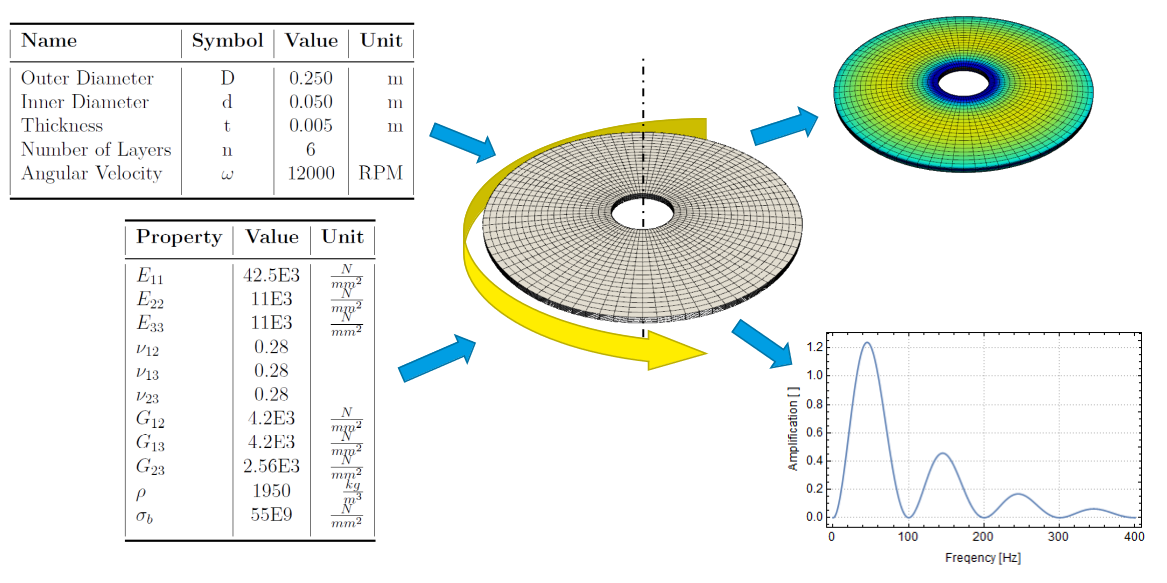
\includegraphics[width=\textwidth]{pics/rotor_model.png}
        \caption{\label{pic:rotor_model} Model of a material lift.}
    \end{subfigure}
    \hfill
    \begin{subfigure}[b]{0.95\textwidth}
        \centering
        \includegraphics[width=\textwidth]{pics/_rotor.pdf}
        \caption{\label{pic:rotor_solution} Implementation of the design process.}
    \end{subfigure}
    \caption{\label{pic:rotor} Designing of a material lift with the introduced framework.}
\end{figure}\\
The interaction of different structural and damage driven optimization criteria, leads to many opportunities for different optimization approaches. 
With eigenfrequency ($f$) and strength  two properties are selected which have negating dependencies to each other (Fig. \ref{pic:rotor_model}),
due to a lower eigenfrequency requiring a lower stiffness.
Reducing the stiffness in a certain layer can only be archived be changing the fiber direction, resulting in a drop of strength.\\
Simulating the development process in the introduced software by 
modelling the material and the rest of the rotor separately, as shown in Figure \ref{pic:rotor_solution}.
This modular approach enables to quickly change the material properties and to reuse the material database.
It further allows to switch easily between different materials and combinations.\\
The generated solutions are grouped as following:
\begin{enumerate}
    \item suitable solutions (principle stress below failure stress ($\sigma_b$))
    \item unsuitable solutions (principle stress over failure stress)
\end{enumerate}
From these two groups only the first suitable solutions are further used.
A fitness value is then computed based on a function which represents the following rules to describe an optimal solution:
\begin{enumerate}
    \item the amount of the principle stress below the failure stress does not matter
    \item a larger distance of the eigenfrequency to the frequency of the engine is better
\end{enumerate}
This was implemented by the following domain-specific fitness-functions.
For the maximum principle stress $\sigma$ evaluation the fitness function is:
\begin{equation}
    \label{eq:fitness_stress}
    f_{\sigma}(\sigma)=2^{(\sigma-\sigma_{b})}=2^{(\sigma-55\frac{N}{mm^2})}
\end{equation}
and with the frequency of the rotor $f_{r}$ being:
\begin{equation}
    \label{eq:rotation_frequency}
    f_{r}=\frac{\omega}{2\pi}=\frac{RPM}{60}
\end{equation}
the fitness function, evaluating the eigenfrequencies, is:
\begin{equation}
    \label{eq:fitness_freq}
    f_{f}(f)=\frac{5 f^5 \exp{\left(-\left((\frac{f}{f_r}\right)^5 + 1\right)}}{5 f_r^5}
\end{equation}
Both domain-specific fitness-functions are then combined to a linear function 
and then scaled separately with the following function:
\begin{equation}
    \label{eq:fitness_final}
    f(\sigma,f)=f_{\sigma}(\sigma)+10f_{f}(f)
\end{equation}
Overall the optimizer tested 56 of 62 possible permutations, which took about 15 min on a normal laptop.
After accounting for creating the model, which took about a week, the new methodology shows a great reduction in work time, 
when compared with the six month which was spend to create \cite{Filippatos2021}.
Some variations could have been reduced, by considering that two layer compositions that can be mapped into each other by mirroring one.
For example the two configurations $[r/r/t/r/r/t]$ and $[t/r/r/t/r/r]$ have similar eigenfrequency and maximum stress.
The cleared permutations are shown with the according stress, eigenfrequency and final fitness score in Figure \ref{pic:rotor_solution}.\\
While the results can vary depending on the used fitness function, the optimum in these particular case is $[r/r/r/t/r/t]$.
With a maximum principle stress $55 \frac{N}{mm^2}$ of and an eigenfrequency of $234 Hz$.\\ 
Repeating the same optimization process with other fitness functions lead to faster results due to majority of cases already computed.
But for larger solutions spaces the break conditions, 
that determine when the optimizer determines if an optimal solution is found,
could be calibrated to reduce the number of computed variants significantly.